% ===================== 担当A =====================
\section{担当A — 指揮者人形・センサ機構}

\subsection{機能一覧}
担当Aでは，楽器ユニット（子機）が演奏を同期させるための指揮者人形ユニット（親機）を開発を担当する．
指揮者人形ユニットは，Arduinoオーケストラにおいて演奏の開始・停止の合図を出し，一定のテンポで腕を振ることで，各楽器ユニット（子機）が同期させるための基準となる役割を担う．\par
本ユニットが担う主な機能は以下の通りである．

\begin{itemize}
    \item \textbf{テンポ提示機能}\\
    腕（反射板）を一定周期で滑らかに往復運動させ，1往復を1拍としてオーケストラ全体のテンポを提示する．

    \item \textbf{拍の同期機能}\\
    腕が最前点に到達した瞬間に，反射板に搭載したLEDを短時間点灯させる．子機は「LEDの光」と「反射板までの距離の変動」の２つの物理的変化を観測することで，通信に頼らず性格に拍を同期する．

    \item \textbf{演奏状態の表現機能}\\
    「待機」「予備拍」「演奏中」「フェルマータ」「演奏停止」の各状態を持ち，状態に応じた動作の変化によって演奏の展開を表現する．

    \item \textbf{外部制御・情報表示機能}\\
    PC上の制御アプリケーションからシリアル通信経由で制御コマンド（START・STOP・FERMATA）を受信する．また．現在の演奏状態を本体のLCDディスプレイに表示し，ユニット単体での状況把握を可能にする．
\end{itemize}

\subsection{システム構成図}
本システムは，ユーザが操作するPC側の制御アプリケーション（Processing），制御と状態管理を担うマイクロコントローラ（Arduino Uno R4 WiFi），および動作と状態提示を行う各出力デバイスによって構成される．
PCからの制御コマンド受信，FspTimerを用いた割り込み処理，およびマイクロ秒単位でのデバイス同期のフローを含む，システム全体の構成図を以下の図\ref{tantoA:system}に示す．

\begin{figure}[H]
    \centering
    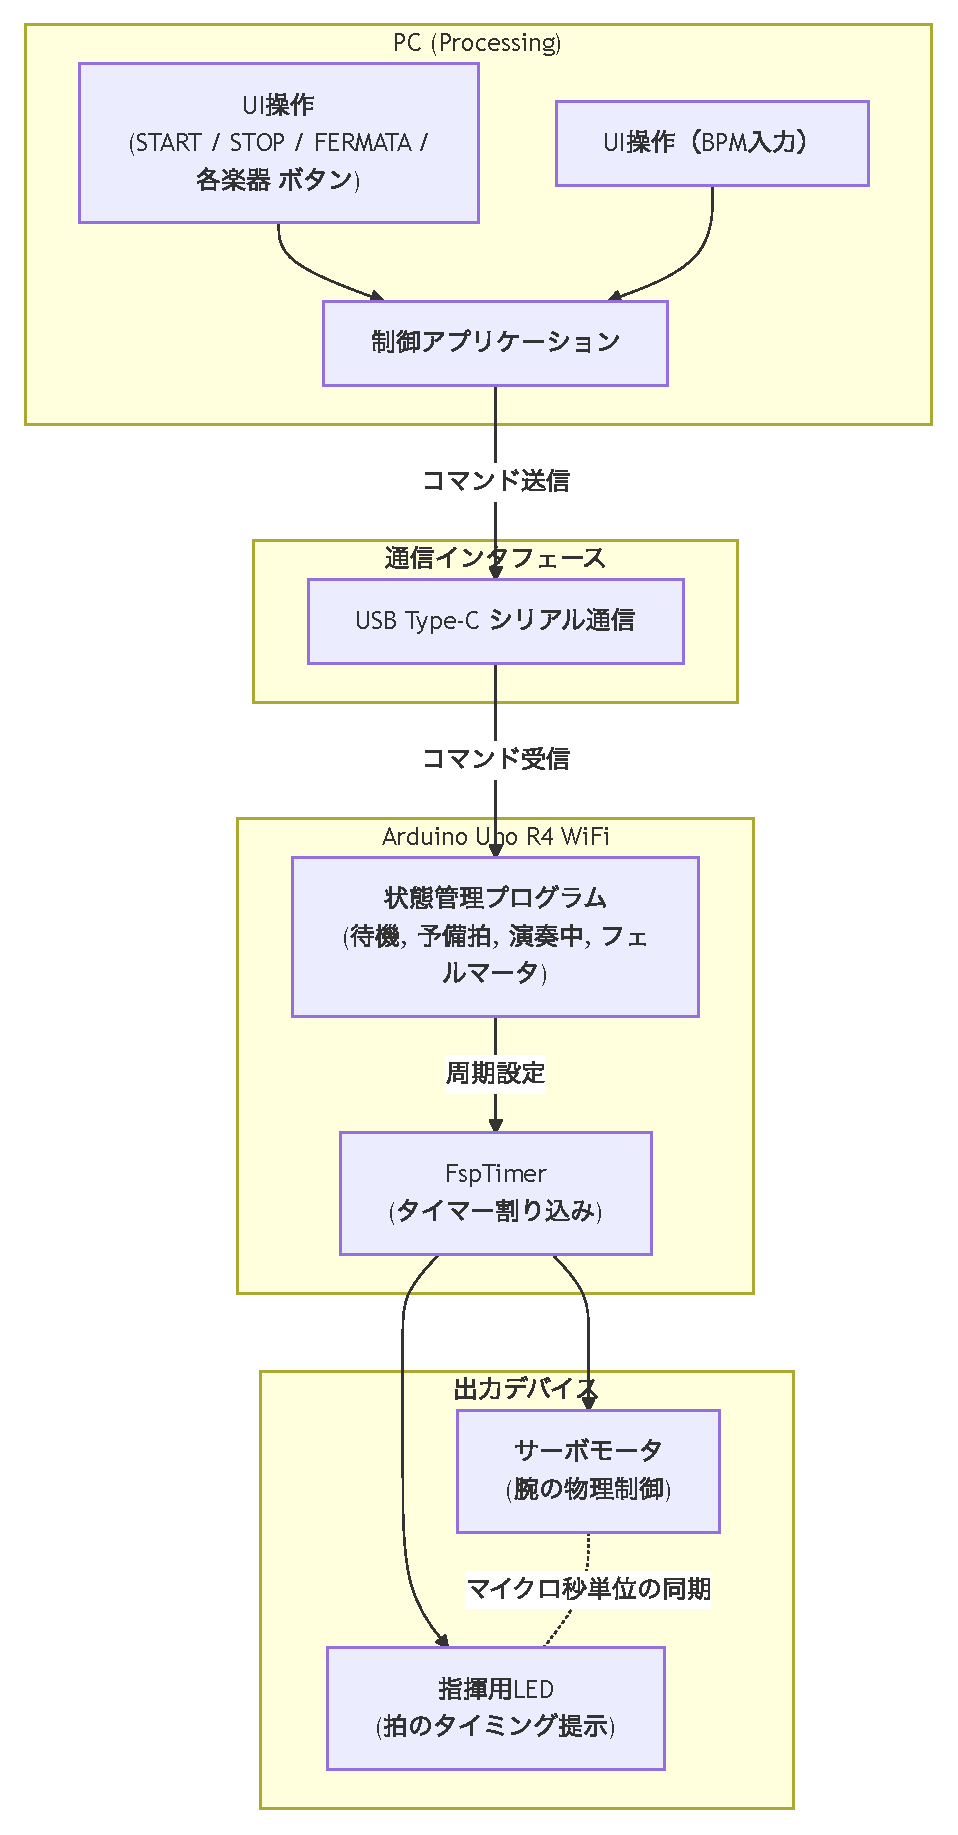
\includegraphics[width=8cm]{figures/tantoA/configuration.pdf}
    \caption{システム構成図}
    \label{tantoA:system}
\end{figure}

\subsection{操作インターフェース設計}
本システムでは，信号入力用の制御アプリケーション（Processingを用いて構築）を介して指揮者人形ユニットの操作を行う．
ユーザインターフェースには，図\ref{tantoA:user}に示すように「START」「STOP」「FERMATA」の各制御ボタンを配置する．
ユーザがPC上でこれらのボタンをクリックすることで，USB Type-Cを用いたシリアル通信を介して，対応する信号がArduinoへ送信される．

\begin{figure}[H]
    \centering
    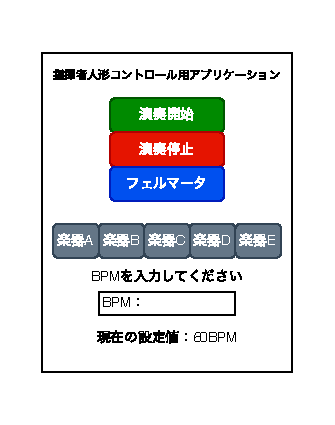
\includegraphics[width=5cm]{figures/tantoA/UI_image.pdf}
    \caption{ユーザーインターフェース表示案}
    \label{tantoA:user}
\end{figure}

\subsection{状態遷移図}
本システムにおける状態遷移図を以下の図\ref{tantoA:flowchart}に示す.

\begin{figure}[H]
    \centering
    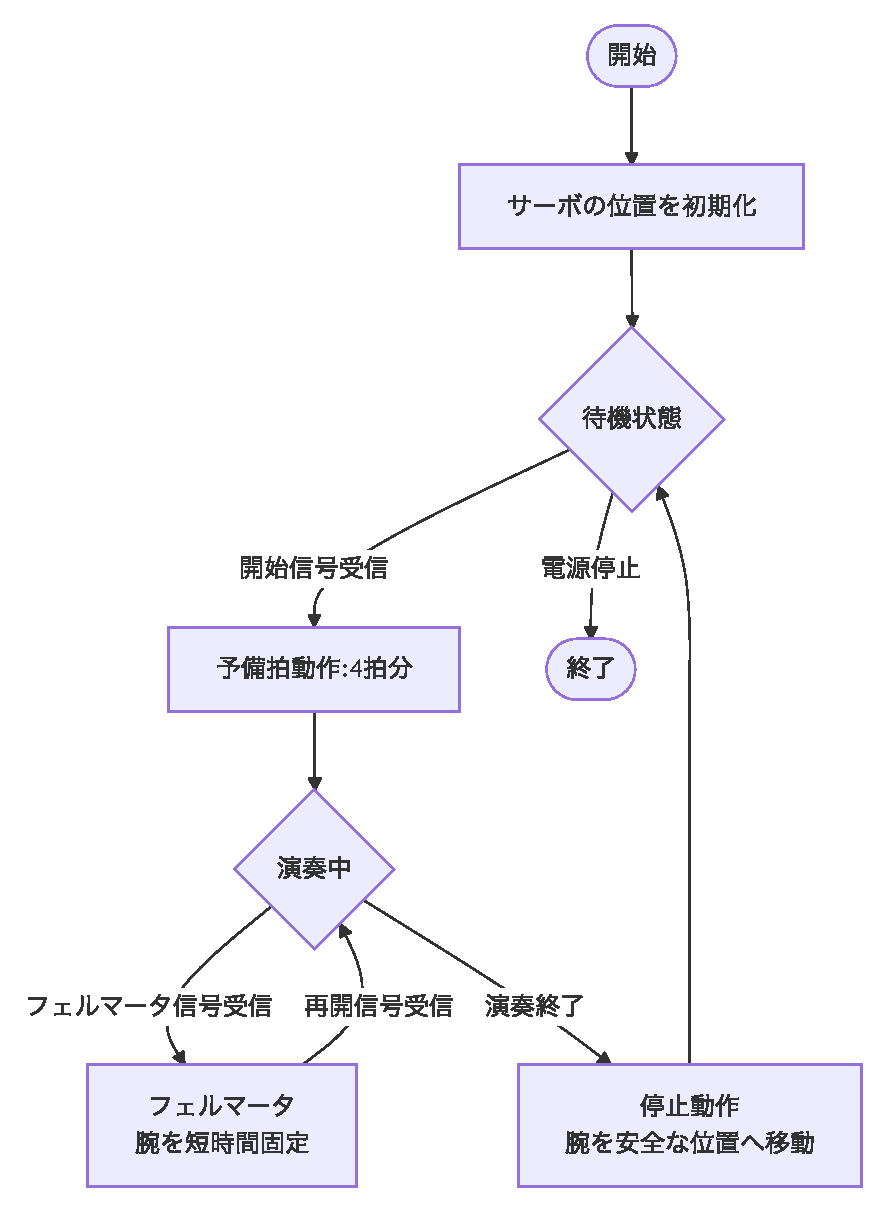
\includegraphics[width=8cm]{figures/tantoA/conductor.pdf}
    \caption{指揮者人形ユニットにおける状態遷移図}
    \label{tantoA:flowchart}
\end{figure}


